\section{Техническое задание}
\subsection{Основание для разработки}

Основанием для разработки является задание на преддипломную (производственную) практику "<Корпоративный портал учета рабочего времени. Серверная часть. На базе ASP.net">.

\subsection{Цель и назначение разработки}

Основной задачей является разработка и внедрение корпоративного портала учета рабочего времени для организации ООО «НОРБИТ».

Посредством внедрения портала, планируется вести учет и контроль рабочего времени сотрудников, отслеживать задачи и проекты пользователей.

Задачами данной разработки являются:
\begin{itemize}
\item создание базы данных с использованием t-sql;
\item написание контроллеров для взаимодействия с интерфейсом программы;
\item реализация логирования под своей учетной записью;
\item реализация взаимодействия с базой данных через внешние URI запросы;
\end{itemize}

\subsection{Требования к программной системе}
\subsubsection{Требования к серверной части программной системы}

Клиентская часть портала должна иметь возможность взаимодействия с серверной часью:
\begin{itemize}
    \item получение данных по URI запросам;
    \item обмен данными через файлы с расширением json;
    \item авторизация пользователей для предоставления доступа к порталу.
\end{itemize}

На рисунке ~\ref{fig:erfdiagdb} представлена концептуальная модель данных программной системы в виде ER-диаграммы сущность-связь.

\begin{figure}[H]
	\centering
	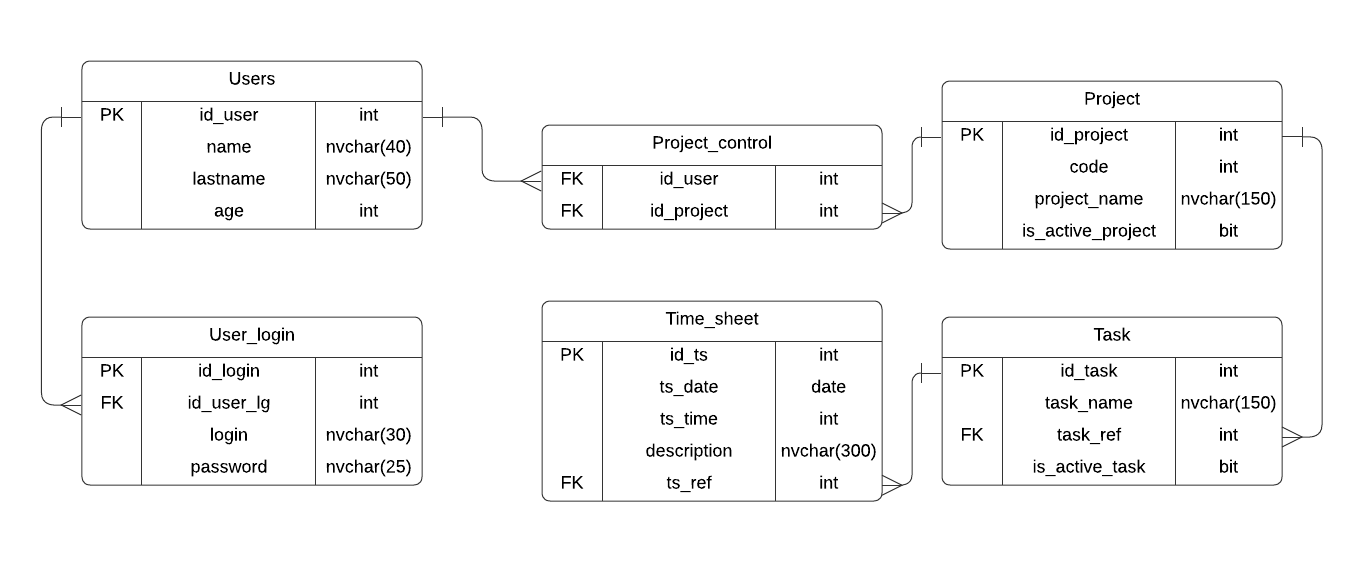
\includegraphics[width=0.9\linewidth]{images/ERFDiagDB}
	\caption{Структура базы данных}
	\label{fig:erfdiagdb}
\end{figure}

Входными данными для портала учета рабочего времени являются:

\begin{itemize}

\item данные о пользователях, включая их имена, фамилии и возраст;
\item учетные данные для авторизации пользователей, такие как логин и пароль;
\item информация о проектах, включая код проекта, название и статус активности;
\item данные о задачах, включая название задачи, ссылку на проект и статус активности;
\item временные данные, включающие дату, время и описание деятельности;
\item контрольные данные, связывающие пользователей с проектами.

Выходными данными являются:

\item отчеты о времени, затраченном на различные проекты и задачи;
\item статистика по активным и завершенным проектам;
\item детализированные записи о выполненных задачах;
\item информация о пользователях, участвующих в различных проектах;
\item данные для авторизации и аутентификации пользователей на портале.
\end{itemize}

\subsubsection{Функциональные требования к программной системе}

В разрабатываемой программно-информационной системе функциональные требования к API предъявляюся со стороны пользовательской части программы.
Должны быть доступны следующие функции программы:

\begin{itemize}
\item Предоставление данных об учетной записи пользователя по логину и паролю.
\item Предоставление данных о проектах, связанных с учетной записью пользователя.
\item Добавление, изменение и редактирование пользовательсих проектов.
\item Предоставление данных о пользовательсих задачах, относящихся к конкретному проекту.
\item Добавление, изменение и редактирование данных о пользовательских задачах.
\item Предоставление данных о проводках, относящихся к конкретной задаче в системе.
\item Добавление, изменение и редактирование данных о проводах.
\item Предоставление данных о проводках за все время и внешними ограничениями с виде промежутка дат.  
\end{itemize}

На рисунке 2.2 в виде диаграммы прецедентов представлены функциональные требования к системее в виде диаграммы прецедентов нотации UML.

\begin{figure}[H]
	\centering
	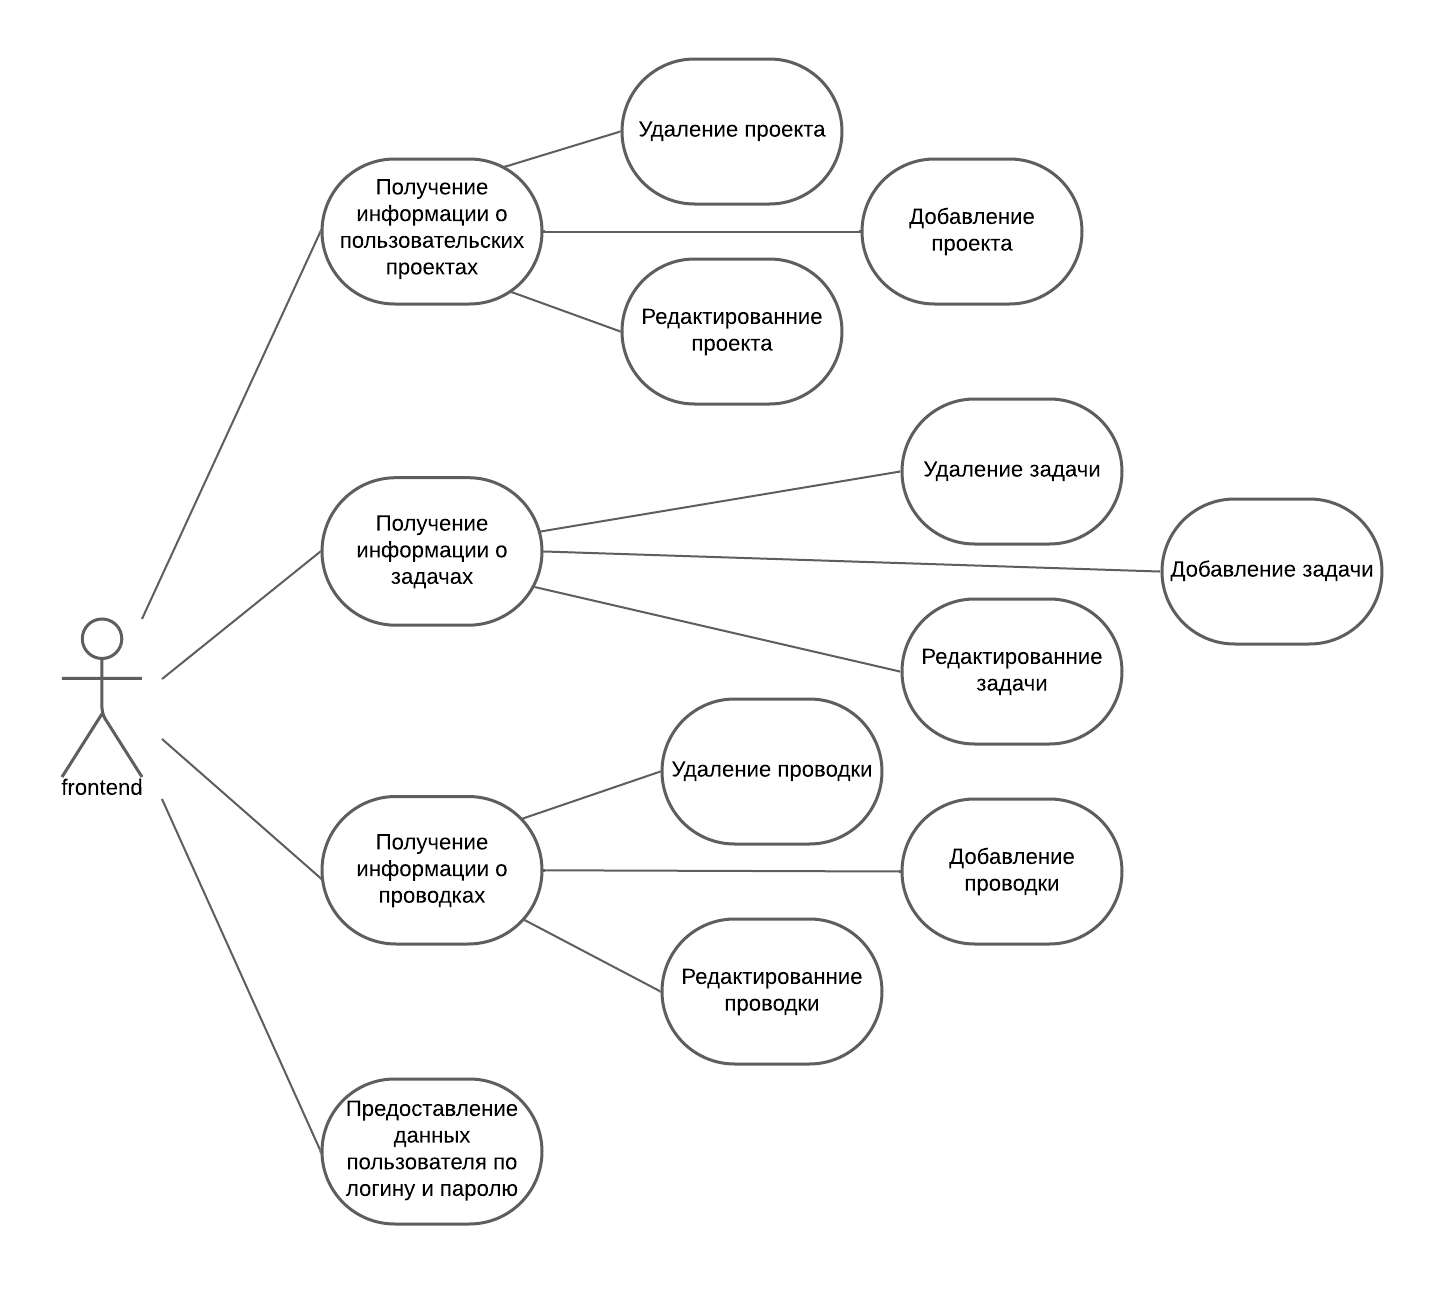
\includegraphics[width=0.9\linewidth]{images/UMLPrecedent}
	\caption{Диаграмма прецедентов}
	\label{fig:umlprecedent}
\end{figure}

\subsubsection{Вариант использования "<Авторизация на веб-портале">}

Заинтересованные лица и их требования: Пользователи веб-портала, которые хотят получить доступ к порталу учета рабочего времени.
Предусловие: Пользователь портала имеет данные для входа от своей учетной записи. Постусловие: Пользователь входит в систему.

Основной успешный сценарий:
\begin{enumerate}
\item Со стороны пользовательской части на сервер отправеляется URI запрос с логином и паролем в формате json файла.
\item Сервер отслеживает запрос и находит пользователя по переданному логину и паролю.
\item Сервер отправляет на frontend json файл с пользовательскими данными.
\end{enumerate}

\subsubsection{Вариант использования "<Получение информации о пользовательских проектах">}

Заинтересованные лица и их требования: Пользователи веб-портала, которые хотят получить доступ к информации о доступных проектах.
Предусловие: Пользователь портала осуществил авторизацию и находится в системе. Постусловие: Пользователь получает данные о проектах.

Основной успешный сценарий:
\begin{enumerate}
	\item Со стороны пользовательской части на сервер отправеляется URI запрос с пользовательским идентификатором в формате json файла.
	\item Сервер отслеживает запрос через контроллер и находит информацию о проектах.
	\item Сервер возвращает на frontend массив всех проектов, доступных данному пользователю.
\end{enumerate}

\subsubsection{Вариант использования "<Добавление нового проекта">}

Заинтересованные лица и их требования: Пользователи веб-портала, которые хотят добаить новый проект под своей учетной записью.
Предусловие: Пользователь портала осуществил авторизацию и находится в системе. Постусловие: Пользователь добавляет новый проект с указанными данными.

Основной успешный сценарий:
\begin{enumerate}
	\item Со стороны пользовательской части на сервер отправеляется URI запрос на добавление проекта с информацией о пользователе.
	\item Сервер отслеживает запрос через контроллер.
	\item Сервер запускает запрос на добавление данных по проекту.
	\item Сервер возвращает на frontend сообщение об успешном добавлении данных по проекту.
\end{enumerate}

\subsubsection{Вариант использования "<Удаление проекта">}

Заинтересованные лица и их требования: Пользователи веб-портала, которые хотят удалить один или несколько доступных проектов.
Предусловие: Пользователь портала осуществил авторизацию и находится в системе. У пользователя есть хотя бы 1 проект. Постусловие: Пользователь удаляет выбранный проект.

Основной успешный сценарий:
\begin{enumerate}
	\item Со стороны пользовательской части на сервер отправеляется URI запрос с кодом проекта, который необходимо удалить в формате json файла.
	\item Сервер отслеживает запрос через контроллер и находит необходимый проект.
	\item Сервер производит каскадное удаление по проекту и всех вложенных данных. 
	\item Сервер возвращает сообщение пользовательской части, об успешном удалении проекта.
\end{enumerate}

\subsubsection{Вариант использования "<Изменение проекта">}

Заинтересованные лица и их требования: Пользователи веб-портала, которые хотят изменить информацию о доступном проекте.
Предусловие: Пользователь портала осуществил авторизацию и находится в системе. У пользователя есть хотя бы 1 проект. Постусловие: Пользователь изменяет выбранный проект.

Основной успешный сценарий:
\begin{enumerate}
	\item Со стороны пользовательской части на сервер отправеляется URI запрос с кодом проекта, который необходимо изменить, а также данные, для изменения выбранного проекта.
	\item Сервер отслеживает запрос через контроллер и находит необходимый проект.
	\item Сервер производит изменение данных по проекту. 
	\item Сервер возвращает сообщение пользовательской части, об успешном изменении проекта.
\end{enumerate}

\subsubsection{Вариант использования "<Получение информации о пользовательских задачах">}

Заинтересованные лица и их требования: Пользователи веб-портала, у которых есть необходимость отслеживать задачи по выбранному проекту.
Предусловие: Пользователь портала осуществил авторизацию и находится в системе. У пользователя есть задачи, относящиеся к конкретному проекту. Постусловие: Пользователь получает данные о задачах по выбранному проекту.

Основной успешный сценарий:
\begin{enumerate}
	\item Со стороны пользовательской части на сервер отправеляется URI запрос с уникальным идентификатором проекта.
	\item Сервер отслеживает запрос через контроллер и находит информацию о задачах.
	\item Сервер возвращает на frontend массив всех задач по выбранному проекту, доступных данному пользователю.
\end{enumerate}

\subsubsection{Вариант использования "<Добавление новой задачи по проекту">}

Заинтересованные лица и их требования: Пользователи веб-портала, которые хотят добаить новую задачу по проекту под своей учетной записью.
Предусловие: Пользователь портала осуществил авторизацию и находится в системе. У пользователя есть хотя бы 1 активный проект. Постусловие: Пользователь добавляет новую задачу по проекту с указанными данными.

Основной успешный сценарий:
\begin{enumerate}
	\item Со стороны пользовательской части на сервер отправеляется URI запрос на добавление задачи с информацией о проекте.
	\item Сервер отслеживает запрос через контроллер.
	\item Сервер запускает запрос на добавление задачи по проекту в соответсвии с переданными данными.
	\item Сервер возвращает на frontend сообщение об успешном добавлении новой задачи.
\end{enumerate}

\subsubsection{Вариант использования "<Удаление задачи по проекту">}

Заинтересованные лица и их требования: Пользователи веб-портала, которые хотят удалить один или несколько доступных задач.
Предусловие: Пользователь портала осуществил авторизацию и находится в системе. У пользователя есть хотя бы одна задача по активному проекту. Постусловие: Пользователь удаляет выбранную задачу.

Основной успешный сценарий:
\begin{enumerate}
	\item Со стороны пользовательской части на сервер отправеляется URI запрос с уникальным идентификатором задачи, которую необходимо удалить.
	\item Сервер отслеживает запрос через контроллер и находит необходимую задачу по проекту.
	\item Сервер производит каскадное удаление по задаче и всех вложенных данных. 
	\item Сервер возвращает сообщение пользовательской части, об успешном удалении задачи.
\end{enumerate}

\subsubsection{Вариант использования "<Редактирование задачи по проекту">}

Заинтересованные лица и их требования: Пользователи веб-портала, которые хотят редактировать информацию о задаче по проекту.
Предусловие: Пользователь портала осуществил авторизацию и находится в системе. У пользователя есть хотя бы одна задача по проекту. Постусловие: Пользователь изменяет выбранную задачу.

Основной успешный сценарий:
\begin{enumerate}
	\item Со стороны пользовательской части на сервер отправеляется URI запрос с уникальным идентификатором задачи, которую необходимо редактировать, а также данные, для изменения выбранной задачи.
	\item Сервер отслеживает запрос через контроллер и находит необходимую задачу.
	\item Сервер производит изменение данных по задаче. 
	\item Сервер возвращает сообщение пользовательской части, об успешном изменении задачи.
\end{enumerate}

\subsubsection{Вариант использования "<Получение данных о проводках по задаче">}

Заинтересованные лица и их требования: Пользователи веб-портала, у которых есть необходимость в просмотра проводок по конкретной задаче.
Предусловие: Пользователь портала осуществил авторизацию и находится в системе. У пользователя есть задачи по проекту и как минимум одна проводка. Постусловие: Пользователь получает данные по проводкам.

Основной успешный сценарий:
\begin{enumerate}
	\item Со стороны пользовательской части на сервер отправеляется URI запрос с уникальным идентификатором задачи, по которой необходимо получить список всех проводок.
	\item Сервер отслеживает запрос через контроллер и находит необходимую задачу.
	\item Сервер запускает скприпт по поиску всех проводок для указанной задачи.
	\item Сервер возвращает список всех проводок по указанной задаче.
\end{enumerate}

\subsubsection{Вариант использования "<Получение данных о проводках за все время">}

Заинтересованные лица и их требования: Пользователи веб-портала, у которых есть необходимость в просмотре проводок за все время.
Предусловие: Пользователь портала осуществил авторизацию и находится в системе. У пользователя есть задачи по проекту и как минимум одна проводка. Постусловие: Пользователь получает данные по проводкам за все время.

Основной успешный сценарий:
\begin{enumerate}
	\item Со стороны пользовательской части на сервер отправеляется URI запрос с уникальным идентификатором задачи, по которой необходимо получить список всех проводок за все время.
	\item Сервер отслеживает запрос через контроллер и находит необходимую задачу.
	\item Сервер запускает скприпт по поиску всех проводок для указанной задачи.
	\item Сервер возвращает список всех проводок за все время.
\end{enumerate}

\subsubsection{Вариант использования "<Добавление новой проводки">}

Заинтересованные лица и их требования: Пользователи веб-портала, у которых есть необходимость в добавлении новой проводки.
Предусловие: Пользователь портала осуществил авторизацию и находится в системе. У пользователя есть задачи по проекту. Постусловие: Пользователь добавляет данные по проводке.

Основной успешный сценарий:
\begin{enumerate}
	\item Со стороны пользовательской части на сервер отправеляется URI запрос с уникальным идентификатором задачи, по которой необходимо добавить проводку.
	\item Сервер отслеживает запрос через контроллер и находит необходимую задачу.
	\item Сервер запускает скприпт на добавление новой проводки, в соотвествии с полученными данными.
	\item Сервер возвращает сообщение на front об успешном добавлении.
\end{enumerate}

\subsubsection{Вариант использования "<Удаление проводки">}

Заинтересованные лица и их требования: Пользователи веб-портала, у которых есть необходимость в удалении проводки.
Предусловие: Пользователь портала осуществил авторизацию и находится в системе. У пользователя есть задачи по проекту и проводки. Постусловие: Пользователь удаляет проводку.

Основной успешный сценарий:
\begin{enumerate}
	\item Со стороны пользовательской части на сервер отправеляется URI запрос с уникальным идентификатором проводки, которую нужно удалить.
	\item Сервер отслеживает запрос через контроллер и находит необходимую проводку.
	\item Сервер запускает скприпт на удаление проводки.
	\item Сервер возвращает сообщение на front об успешном удалении.
\end{enumerate}

\subsubsection{Вариант использования "<Редактирование проводки">}

Заинтересованные лица и их требования: Пользователи веб-портала, у которых есть необходимость в редактировании проводки.
Предусловие: Пользователь портала осуществил авторизацию и находится в системе. У пользователя есть задачи по проекту и проводки. Постусловие: Пользователь редактирует проводку.

Основной успешный сценарий:
\begin{enumerate}
	\item Со стороны пользовательской части на сервер отправеляется URI запрос с уникальным идентификатором проводки, которую нужно редактировать, а так же данные на осонове которых происходит изменение через json файл.
	\item Сервер отслеживает запрос через контроллер и находит необходимую проводку.
	\item Сервер запускает скприпт на редактирование проводки.
	\item Сервер возвращает сообщение на front об изменении проводки.
\end{enumerate}


\subsection{Нефункциональные требования к программной системе}
\subsubsection{Требования к архитектуре}
Серверная часть портала должна быть написана с использованием концепции mvc. База данных должна находится отдельно от файлов проекта для гарантирования целостности данных. Взаимодействие между пользовательской и серверной частью портала должна быть осущестлена по URI запросам с использование протокола HTTPS. Отправка данных должна осуществляться через файлы с расширением .json.

\subsubsection{Требования к безопасности и надежности данных}
Сервер базы данных должен быть написан на языке запросов Microsoft SQL. Сама база данных не должна находится каталогах самого проекта. Подключение к базе данных должно осуществляться через промежуточный файл secret.json, в котором хранится строка подключения к БД. Для обеспечения целостности и предотвращения утечки данных, необходима реализация каскадного удаления, а так же использование транзакций. 

Портал должен выдерживать до 100 запросов в секунду.

\subsubsection{Требования к программному обеспечению}

Для реализации backend части корпоративного портала должны использоваться
следующие технологии:
\begin{itemize}
	\item язык программирования C\#;
	\item библиотека ASP.net MVC.
\end{itemize}

\subsubsection{Требования к аппаратному обеспечению}

Для работы backend части веб-платформы на ASP.NET MVC с использованием Microsoft SQL Server необходим сервер на операционной системе Windows Server. Рекомендуется наличие установленного .NET Framework и SQL Server. Требуется процессор с частотой не менее 2.5 GHz и многопоточностью, дисковое пространство не менее 20 Гб для хранения данных и файлов проекта, а также свободная оперативная память в размере не менее 8 Гб для обеспечения быстрой и стабильной работы приложений. Видеокарта в данном случае не обязательна, так как нагрузка на графический процессор минимальна.

\subsubsection{Требования к оформлению документации}

Разработка программной документации и программного изделия должна производиться согласно ГОСТ 19.102-77 и ГОСТ 34.601-90. Единая система программной документации.
